\documentclass[a4paper, 11pt]{article} % Font size (can be 10pt, 11pt or 12pt) and paper size (remove a4paper for US letter paper)

\usepackage[protrusion=true,expansion=true]{microtype} % Better typography
\usepackage{graphicx} % Required for including pictures
\usepackage{wrapfig} % Allows in-line images
\usepackage{listings} % Allows code listing
\usepackage{float} % Allow holding images in place
\parskip = \baselineskip % skip lines between paragraphs

\usepackage{mathpazo} % Use the Palatino font
\usepackage[T1]{fontenc} % Required for accented characters
\linespread{1.05} % Change line spacing here, Palatino benefits from a slight increase by default

\makeatletter
\renewcommand\@biblabel[1]{\textbf{#1.}} % Change the square brackets for each bibliography item from '[1]' to '1.'
\renewcommand{\@listI}{\itemsep=0pt} % Reduce the space between items in the itemize and enumerate environments and the bibliography

\renewcommand{\maketitle}{ % Customize the title - do not edit title and author name here, see the TITLE block below
\begin{flushright} % Right align
{\LARGE\@title} % Increase the font size of the title

\vspace{30pt} % Some vertical space between the title and author name

{\large\@author} % Author name
\\\@date % Date

\vspace{30pt} % Some vertical space between the author block and intro
\end{flushright}
}

%----------------------------------------------------------------------------------------
%	TITLE
%----------------------------------------------------------------------------------------

\title{\textbf{ECS 145 Term Project Report}\\ % Title
DES implementations in R and Python} % Subtitle

\author{\textsc{Peter Van Ausdeln, Henry Jue, Niklas Kraemer} % Author
\\{\textit{UC Davis}}} % Institution

\date{\today} % Date

%----------------------------------------------------------------------------------------

\begin{document}

\maketitle % Print the title section

%----------------------------------------------------------------------------------------
%	ABSTRACT AND KEYWORDS
%----------------------------------------------------------------------------------------

%----------------------------------------------------------------------------------------
%	ESSAY BODY
%----------------------------------------------------------------------------------------

\section*{Introduction: What is DES?}

Discrete Event Simulation (DES) is a way of modelling a system and the events that occur within said system. To be a valid system for DES, the events of this system must occur in distinct blocks of time. The average number of points scored by a basketball player over the course of his season would be a valid use of DES. Each game is a discrete event, and each set of points is a discrete number. The changes in wind speed in a certain location would, on the other hand, not be a valid use of DES.


To model DES with a programming language package or library, the package must have specific functionality. First, it must be able to simulate a given length of time. This will allow the package to accumulate data from the events as they occur over time. One way of doing this involves storing a time variable and a time limit variable in the class. To simulate passing time, the package incremented the time variable at certain points, and ends the simulation when the time variable passes the time limit variable.


The package must also be able to decide when the events occur during that time. Packages usually do this through keeping a schedule of events, often in a queue. When the simulated time of the package reaches the time that the event is scheduled to occur, the event is popped from the queue, handled, and data is gathered from it. This schedule allows the code, in some implementations, to handle the passing of time through a step function. This involves incrementing the stored "current time" to the time of the next event, after the previous event is completed. Since nothing is scheduled to happen between those two times, that time can be safely skipped over.


The package must also have code to simulate the popped event happening, using any parameters it is given. Without the ability to specify event parameters, such as frequency and magnitude, the user has no flexibility in using the program and likely will not be able to get the data needed for analysis. The package must also be able to calculate and deliver the desired analysis to the user. In the basketball example, that might be the average and standard deviation of points scored per game. For the warehouse example, it might be the same statistics for the average number of items in the warehouse. If the package can record the data, but cannot do anything productive with it, its usefulness drops.


There are three main methods used to implement the skeleton of DES. These methods focus on different aspects of the DES model. They are activity-based, process-oriented, and event-oriented. In this report we will discuss the process-oriented and event-oriented methodS.


%------------------------------------------------

\section*{Event-Oriented DES}

Often, the simplest way of implementing DES is to make it event-oriented. Many of the possible implementations of different parts of DES discussed in the previous section are used in Event-Oriented DES. We see one full implementation of an Event-Oriented DES skeleton in the DES.R example (see code listing at the end). As implied by the name, Event-Oriented DES, and by extension DES.R, bases its simulation on handling each event in sequence. 

One of the major aspects of Event-Oriented DES is its use of shortcuts in its simulated time-frame. It uses these shortcuts to skip to each new event that it must track. This is where the event list comes in handy. A known event is scheduled and put into the list. When this happens in the course of the simulation is left to the user. After one event finishes, the system moves to the time of the next event. Since we know that the given event is the next event to happen, we know that no events of consequence will occur in the times that we skip. Therefore, it is safe to skip those times. The skip-time algorithm works essentially as follows: \pagebreak

\begin{lstlisting}[caption=Skip Time Algorithm]
	nextEventTime = eventQueue.front.eventTime
	if(nextEventTime < endSimTime)
		currentSimTime = nextEventTime
	else
		exit()
\end{lstlisting}
We see another example of this in DES.R. See the code labelled "skipTime" for the exact time-skipping code in the package. Sometimes, we need extra functionality regarding the priority of different kinds of events (such as in a natural disaster simulation). In these cases, we use a priority queue instead of a simple list. DES.R specifically uses a matrix to simulate a queue.

Once the Event-Oriented DES is at the next event time, it must handle the event. In many cases, this may involve multiple events, so the system must have a way of knowing which event is about to occur. DES.R makes a framework for this through its "evnttype" variable, in which each type of event is given a different identifier. As we see in the code labeled "eventAdd", this information goes into the event queue along with the event itself. It also uses a user-supplied "reactevent" as the specific event handler (as clearly the handler will need to be changed for specific uses of the library, see "eventHandleReact" code section). 

The general algorithm for Event-Oriented DES is simple. While there's still an event scheduled to happen within the time limit, we skip to the next event and call the event handler. As opposed to Process-Oriented DES, this is much easier to implement (avoided threads) and often works faster, especially because most of the simulation time is skipped over. \pagebreak

%------------------------------------------------

\section*{Process-Oriented DES}

Often, the simplest way of implementing DES is to make it event-oriented. Many of the possible implementations of different parts of DES discussed in the previous section are used in Event-Oriented DES. We see one full implementation of an Event-Oriented DES skeleton in the DES.R example (see code listing at the end). As implied by the name, Event-Oriented DES, and by extension DES.R, bases its simulation on handling each event in sequence. 

One of the major aspects of Event-Oriented DES is its use of shortcuts in its simulated time-frame. It uses these shortcuts to skip to each new event that it must track. This is where the event list comes in handy. A known event is scheduled and put into the list. When this happens in the course of the simulation is left to the user. After one event finishes, the system moves to the time of the next event. Since we know that the given event is the next event to happen, we know that no events of consequence will occur in the times that we skip. Therefore, it is safe to skip those times. The skip-time algorithm works essentially as follows: 

We see another example of this in DES.R. See the code labeled "SKIP TIME" for the exact time-skipping code in the package. Sometimes, we need extra functionality regarding the priority of different kinds of events (such as in a natural disaster simulation). In these cases, we use a priority queue instead of a simple list. DES.R specifically uses a matrix to simulate a queue.

Once the Event-Oriented DES is at the next event time, it must handle the event. In many cases, this may involve multiple events, so the system must have a way of knowing which event is about to occur. DES.R makes a framework for this through its "evnttype" variable, in which each type of event is given a different identifier. As we see in the code labeled "EVENT ADD", this information goes into the event queue along with the event itself. It also uses a user-supplied "reactevent" as the specific event handler (as the handler will need to be changed for specific uses of the library, see "REACT EVENT" code section). 

The general algorithm for Event-Oriented DES is simple. While there's still an event scheduled to happen within the time limit, we skip to the next event and call the event handler. As opposed to Process-Oriented DES, this is much easier to implement (avoided threads) and often works faster, especially because most of the simulation time is skipped over.\pagebreak

\begin{figure}[H]
	\caption{DES.R Code Part 1}
	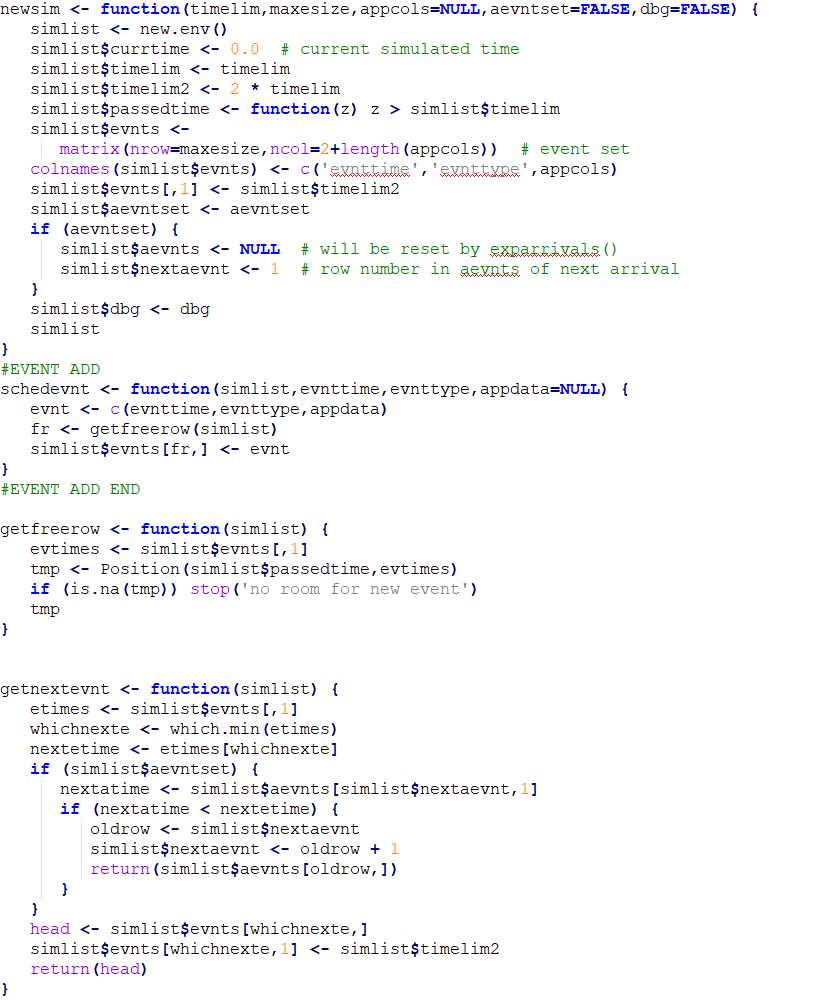
\includegraphics{des1}
	\centering
\end{figure} \pagebreak

\begin{figure}[H]
	\caption{DES.R Code Part 2}
	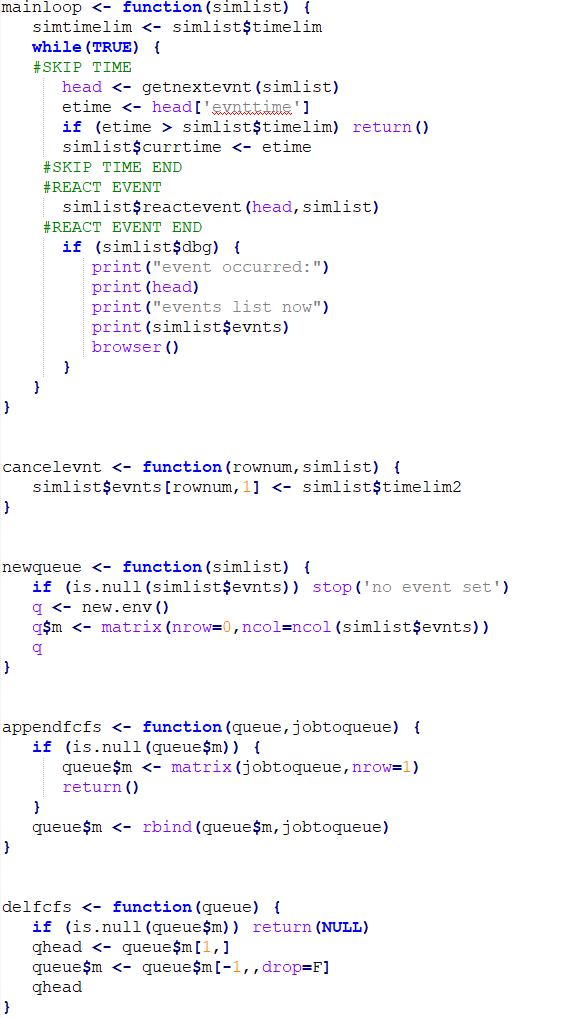
\includegraphics{des2}
	\centering
\end{figure} \pagebreak

\begin{figure}[H]
	\caption{DES.R Code Part 3}
	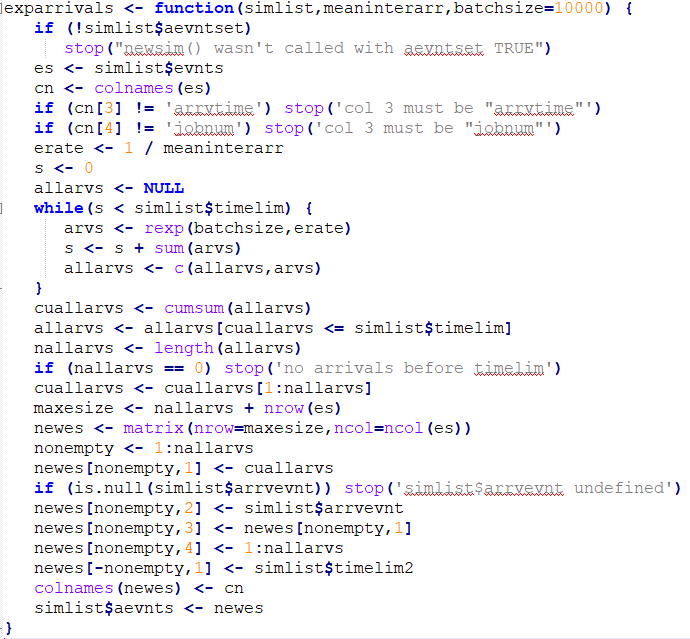
\includegraphics{des3}
	\centering
\end{figure} \pagebreak

%------------------------------------------------

\section*{Rposim Package}

Rposim stuff will go here. \pagebreak

%------------------------------------------------

\section*{Simmer Package}

"Simmer" is another R package that has the same basic functionality as Rposim. It is also designed as a process-oriented DES package. It is advertised as being like Simpy. However, Simpy uses generators as the backbone of its process handling. R does not have generators, or even multithreading capability. How then does Simmer work as a "process-oriented" package? As we look through the different ways that Simmer makes process-oriented DES work, we will go over an example of the package in use, using a very similar simulation model to MachRep.R. The code will be listed at the end of this section.

There are some parts of simmer that work effectively in an identical manner to Simpy. First, Simmer encapsulates the entire simulation within a single "environment", built by the \texttt{simmer}() function (line 12 in the example code). As we can see in the rest of the code, everything else that we build for the simulation is attached to that environment (simply named "env" in the example). Simmer also uses a \texttt{run}() function to simulate the passing of time, accepting a number parameter to serve as the stopping point (line 35). Note that we attached this run function to the already-built "env" environment, as with everything else built for the simulation. However, though there are similarities between Simpy and Simmer, there are still bound to be major differences since Simmer cannot exploit Python's generators and multithreading capabilities.

There are a few methods that Simmer uses to overcome these issues in building its package. The first one is rather simple. It builds its own version of Python generators. Each generator defines the inner workings of one "object" in each simulation. We can see that in lines 28-29 of our sample code, each generator is hooked up to one of the machines that will be running, along with what time it will start (at(0)), how much monitoring will be done (mon=2), and the exact function that each machine will perform during the simulation (runMach(i)). We build one generator for each object in the loop. \pagebreak

The \texttt{runMach} function is the meat of this simulation. It is where all the interesting stuff happens and where all the data is collected. To make these functions work, Simmer exploits the concept of a "trajectory". A trajectory is a set of actions that are linked together into a chain, using the \%>\% functionality from the magrittr package, where they build off each other. By combining this chain of actions with the \texttt{rollback} function, we can both tell the machine generator what to do, and to repeat it ad nauseum until the simulated time is up. The \texttt{rollback} function takes two numbers. The first tells the trajectory how many commands to "roll back", while the second one tells when to repeat that rollback. In our use (line 24), we roll back 6 lines (to the first timeout) and repeat that an infinite number of times. The rollbacks end when the simulated time is up.


The trajectory also contains Simmer's methods of data collection. We decide what data we want to collect in the trajectory and then record it as necessary using "attributes". Specifically, we use the \texttt{set\_attribute} function. In our machine repair, we track two variables, the total up time of a machine, and the number of repairs. At the end of the program, in lines 37-40, we print out the monitored attributes, using the \texttt{get\_mon\_attributes} function. Each generator has its own copies of (and values assigned to) the used attributes. Simmer likes to take advantage of the dplyr data manipulation package to format some of its prints.

\begin{figure}[H]
	\caption{Simmer Excerpts from MachRep (in order of mention)}
	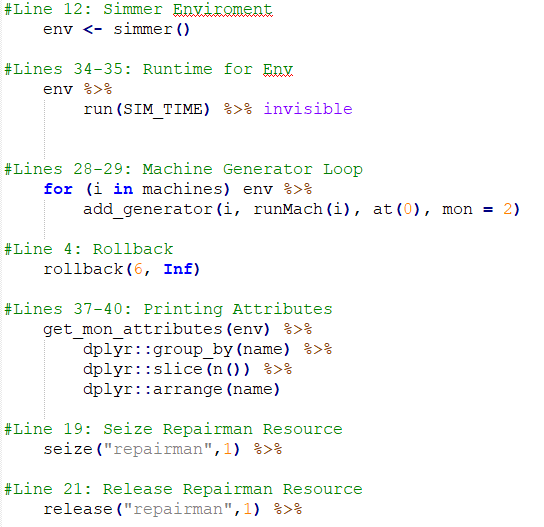
\includegraphics{simmer1}
	\centering
\end{figure} \pagebreak

\begin{figure}[H]
	\centering
	\caption{Full Simmer MachRep Implementation}
	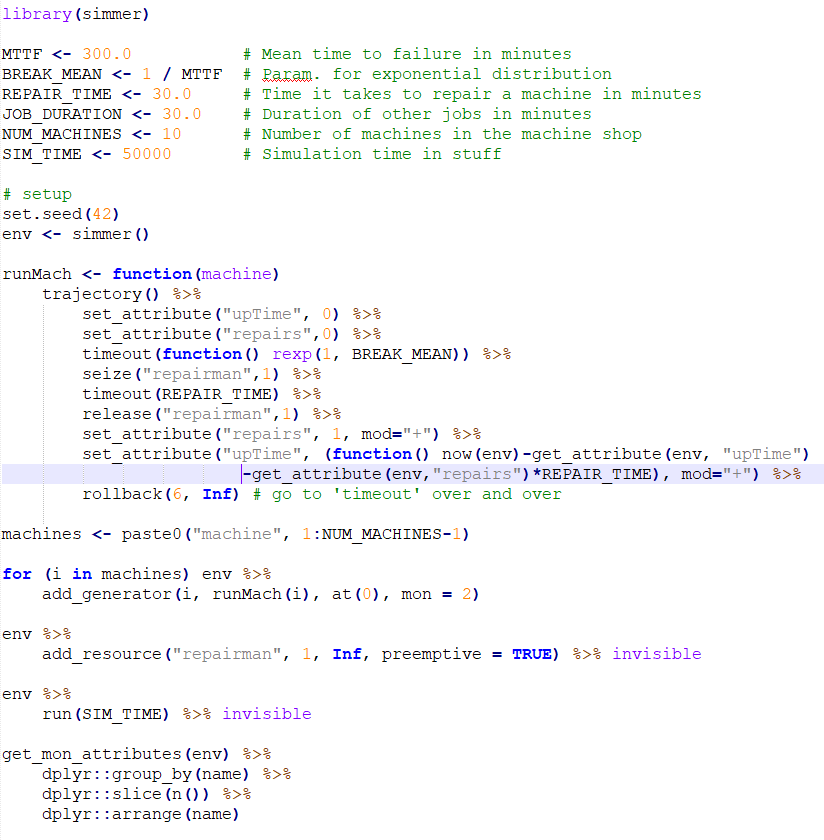
\includegraphics[width=16cm]{simmer2}
\end{figure} \pagebreak

\end{document}